\section{Pipeline}

\begin{frame}[fragile]
  \frametitle{Pipeline}
\begin{center}
 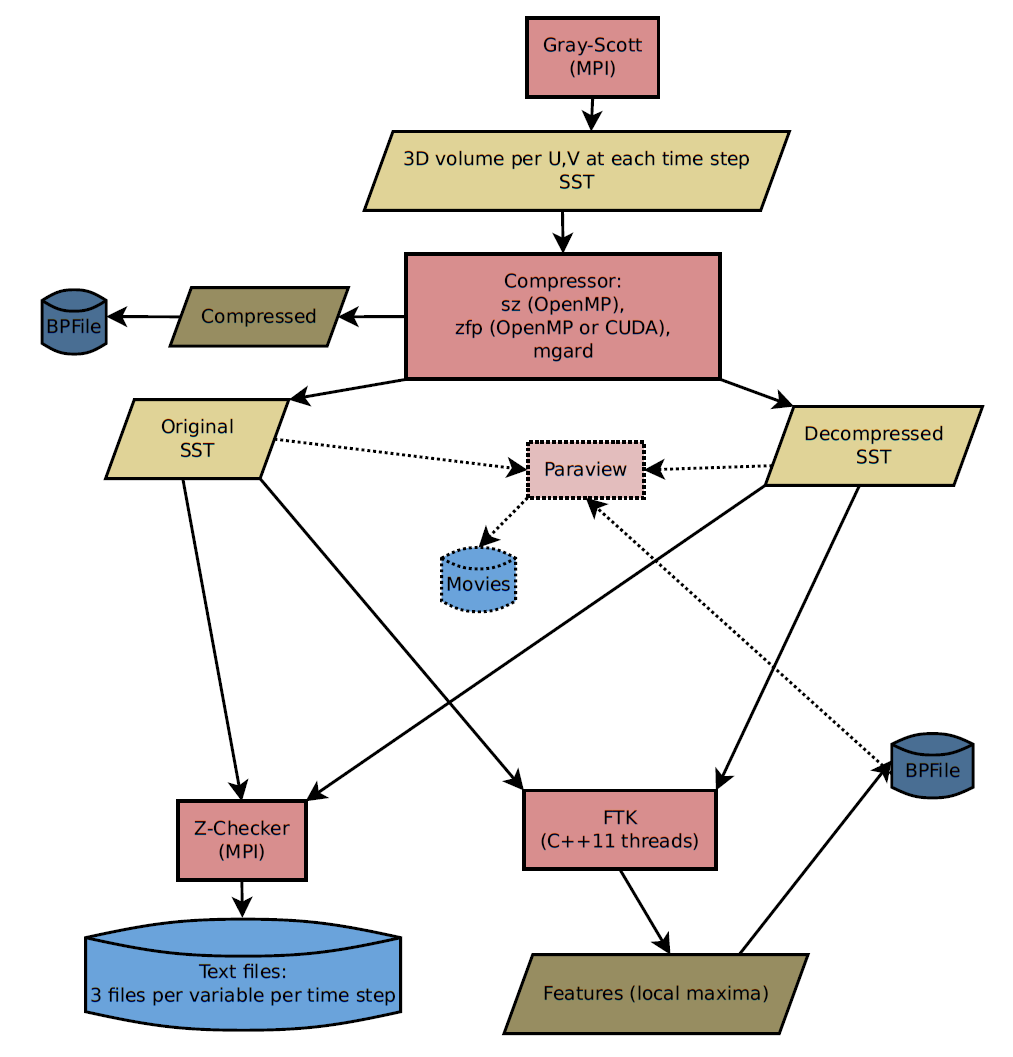
\includegraphics[width=7.6cm]{graphs/pipeline.png}
\end{center}
\end{frame}


\begin{frame}[fragile]
  \frametitle{Pipeline}
  \begin{itemize}
  \item Gray-Scott simulation
    \begin{itemize}
    \item currently uses $256^3$ grid
    \item two variables, $U$ and $V$, evolve according to two coupled non-linear PDEs, generating non-trivial patterns
    \item initial condition: $U$ is 1 everywhere except for the cube in the middle where it is 0.25; $V$ is 0 everywhere except for the
      same cube in the middle where it is 0.33
    \item some random noise is added to $U$ at each iteration, its amplitude is a parameter
    \item 1000 time steps
    \item every 100 steps a checkpoint is created and sent via ADIOS2 SST stream to compressor
    \end{itemize}
  \end{itemize}
\end{frame}

\begin{frame}[fragile]
  \frametitle{Pipeline}
  \begin{itemize}
  \item Compressor
    \begin{itemize}
    \item uses one of the following algorithms: SZ, ZFP, MGARD
    \item compresses and decompresses the data
    \item compressed data is written to a file with enough metadata to decompress
    \item original and lossy (compressed/decompressed) data are sent via ADIOS2 SST streams to ZChecker and FTK to evaluate the quality of the compression
    \end{itemize}
  \item ZChecker
    \begin{itemize}
    \item gets original and lossy data
    \item runs its usual comparison and stores the results in usual ZChecker format: 3 text files per iteration, per variable
    \end{itemize}
  \end{itemize}
\end{frame}

    
\begin{frame}[fragile]
  \frametitle{Pipeline}
  \begin{itemize}
  \item FTK
    \begin{itemize}
    \item gets original and lossy data
    \item finds the number of local maxima on each variable on both datasets
    \item computes the distance as normalized difference between the number of local maxima for each variable
    \item local maxima coordinates and values, number of maxima, distances are stored in ADIOS2 BP4 files.
    \end{itemize}
  \item Cheetah/Savanna is used to set up and run the experiments
  \item ParaView
    \begin{itemize}
    \item used for debugging purposes offline
    \item compared original and lossy data side by side to visualize time evolution and spacial distribution of $U$ and $V$
      and show local maxima found by FTK
    \item see the link to movies on $32^3$ grid in references
    \end{itemize}
  \end{itemize}
\end{frame}

    
